
\chapter{Errore Umano}

La maggior parte degli incidenti industriali è causata da errore umano:
le stime si aggirano tra il 75\% e il 95\% del totale.

\begin{flushleft}
	\textit{Come è possibile che tante persone siano così incompetenti?}
\end{flushleft}

La risposta è semplice! Non lo sono, il problema è nella mal progettazione e nel cattivo design.

Si continuano a produrre dispositivi e software che richiedono, a chi li usa, di mantenere per ore un'attenzione ed una vigilanza complete, oppure di memorizzare procedure arcaiche, confuse e usate di rado, magari anche una sola volta nella vita. Si costringono le persone a stare in un ambiente monotono senza nulla da fare per ore e ore, salvo dovere improvvisamente rispondere con rapidità e precisione. Le si sottopone ad un ambiente di lavoro complesso e sovraccarico, dove sono continuamente interrotte durante l'esecuzione di compiti simultanei. L'\textbf{interruzione è una delle cause che più frequentemente portano all'errore umano}.

Uno dei più grandi \textbf{problemi} è l'\textbf{atteggiamento delle persone verso gli errori} commessi. Quando un errore causa perdite economiche o, peggio ancora, danni alle persone, si istituisce una speciale commissione d'inchiesta, che quasi immancabilmente trova i colpevoli.

Il passo successivo è punirli con multe, il licenziamento o addirittura il carcere. Essi vengono incolpati
e puniti o, nella migliore delle ipotesi, incolpati e riaddestrati. Tutto questo però non
risolve il problema: lo \textbf{stesso errore continuerà a presentarsi}.  Per evitare di incorrere nuovamente nell'errore, quando esso viene commesso, è bene  studiarne le cause, per poi ridisegnare il prodotto o le procedure in modo che esso non si ripeta o, se dovesse ripetersi, che i danni siano ridotti al minimo.

\section{Root Cause Analysis}
La \textbf{Root Cause Analysis} consiste nell'indagare l'incidente finché non si trova la singola causa che ne è l'origine. Ovvero il momento nel tempo quando effettivamente qualcuno ha preso decisioni o eseguito azioni sbagliate e,
una volta fatto ciò, accertare da cosa è derivato lo sbaglio. Purtroppo, troppo spesso, il processo si ferma non appena si scopre che una persona ha agito in maniera impropria, additandola come \textit{colpevole}.

Cercare di trovare la causa di un incidente suona bene, ma ha due difetti.

\begin{enumerate}
	\item La maggior parte degli incidenti \textbf{non ha una sola causa}. Da qui il \textbf{modello a groviera degli incidenti} di James Reason.
	\item Solitamente l'analisi delle cause profonde si ferma non appena trovato un errore umano.
\end{enumerate}

\pagebreak

\begin{figure}[!h]
	\centering
	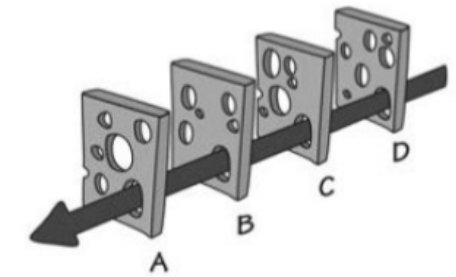
\includegraphics[scale=0.55]{immagini/Groviera.png}
	\caption{Modello a groviera.}
\end{figure}

Se una macchina smette di funzionare per un guasto o un malfunzionamento
si cerca di capire come mai si è rotta o cosa l'ha portata a guastarsi. È
opportuno fare lo stesso quando si scopre un errore umano: \textbf{individuarne le cause}.

Quando durante l'analisi delle cause profonde si incontra, nella concatenazione di cause ed effetti, un errore umano, \textbf{il lavoro è appena cominciato}: bisogna capire \textbf{perché} l'errore \textbf{è accaduto e cosa si può fare per prevenirlo}.

\section{I cinque perchè}

L'analisi delle cause profonde mira a determinare la causa \textbf{prima di un evento}, non la causa immediata.

In Giappone da tempo si usa a questo scopo una procedura detta \textit{"dei \textbf{cinque perché}"} ideata da Sakichi Toyoda e impiegata dalla Toyota nell'ambito del sistema di controllo qualità dei suoi prodotti.

Fondamentalmente quindi quando si cerca la ragione di un evento non ci si deve fermare dopo averne trovata solo una, ma bisogna continuare ad indagare fino a che non si trovano le \textbf{vere cause di fondo}.

Va ripetuta davvero cinque volte?

No, ma chiamarla \textit{procedura dei cinque perché} sottolinea la necessità di proseguire anche dopo aver trovano una causa apparente.

Vediamo un esempio: \textbf{il veicolo non si accende}.

\begin{enumerate}
	\item \textbf{Perché?} La batteria è morta.
	\item \textbf{Perché?} L'alimentatore non funziona.
	\item \textbf{Perché?} La cinghia dell'alternatore non funziona.
	\item \textbf{Perché?} La cinghia dell'alternatore era ben oltre il suo tempo di servizio e non è stata sostituita.
	\item \textbf{Perché?} Il veicolo non è stato mantenuto secondo le tempistiche raccomandate.
\end{enumerate}

Quando le persone sbagliano, bisogna \textbf{cambiare il sistema} in modo da evitare l'errore
e, se non è possibile eliminarlo del tutto, almeno fare in modo di ridurne gli effetti.

Se il sistema lascia sbagliare gli utenti è \textbf{mal progettato}, se il sistema induce all'errore, allora è \textbf{progettato malissimo}.

\pagebreak

\begin{flushleft}
	\textit{Perchè le persone sbagliano?}
\end{flushleft}

Perchè il design si concentra sulle esigenze del sistema
e delle macchine, non su quelle degli utenti. Le macchine hanno bisogno in genere di
comandi precisi, obbligando l'operatore a introdurre esatte informazioni numeriche. Gli esseri umani non sono adatti ad esercitare grande precisione e commettono spesso
errori quando devono digitare lunghe sequenze di numeri o lettere.

Gli umani sono creativi, curiosi, costruttivi, particolarmente bravi nel creare modi nuovi di fare le cose e nel cogliere nuove opportunità. Compiti monotoni, ripetitivi e precisi contraddicono tali qualità e vi entrano in conflitto.

\section{Definizione di errore}
Si definisce \textbf{errore umano} ogni deviazione dal comportamento \textit{appropriato}. Il termine appropriato è da prendere con le pinze, perché in molte circostanze si scopre quale fosse il comportamento giusto solo successivamente.

Generalmente comunque si chiama \textit{errore} ogni comportamento che si discosta da quello generalmente accettato come giusto o adeguato. \textbf{Errore} è il termine generale per tutte le situazioni sbagliate. È possibile dividere gli errori in \textbf{due} classi:

\begin{multicols}{2}
	\centering
	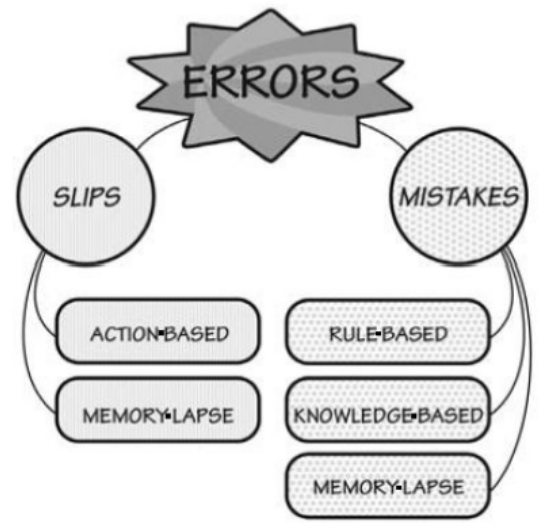
\includegraphics[scale=0.25]{immagini/Errors.png}
	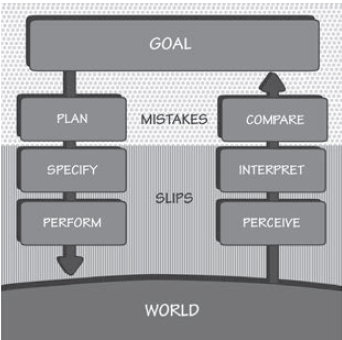
\includegraphics[scale=0.4]{immagini/Errors1.png}
\end{multicols}

\begin{enumerate}
	\item \textbf{Lapsus o Slips}: si ha un lapsus quando s'intende eseguire un'azione e si finisce per eseguirne un'altra. Nel caso del lapsus, l'azione eseguita non è quella voluta. Ci sono \textbf{due tipi principali di lapsus}:
	      \textbf{lapsus di azione e lapsus di memoria}.
	      Nel primo caso si esegue un'azione sbagliata, nel secondo si dimentica di eseguire
	      l'azione o di valutarne i risultati.
	      Esempio di \textbf{lapsus di azione}: versare il latte nel caffè e poi riporre la tazza in frigorifero. L'azione è giusta ma è applicata all'oggetto sbagliato.
	      Esempio di \textbf{lapsus di memoria}: dimenticare di spegnere il fornello dopo aver terminato la cottura. \textbf{I lapsus si hanno nelle fasi attuative e percettive dell'azione.}
	\item \textbf{Errori cognitivi o Mistakes}: si ha un errore cognitivo quando è sbagliato il goal o lo scopo: da quel momento in poi le azioni, anche se eseguite a puntino, fanno parte dell'errore essendo di per sé inappropriate, in quanto parte di un progetto sbagliato. In questo tipo di errore l'azione è corretta ma l'intenzione no.
	      Gli errori cognitivi si suddividono in: \textbf{regola sbagliata}, \textbf{conoscenza sbagliata e dimenticanza}. In un errore generato dall'applicazione della \textbf{regola sbagliata}, la
	      diagnosi della situazione è giusta, ma poi viene scelto un corso d'azione sbagliato,
	      seguendo una regola operativa errata. In un errore causato da \textbf{conoscenza erronea}
	      o \textbf{incompleta}, ad essere sbagliata è la diagnosi stessa della situazione. Gli errori per \textbf{dimenticanza} si hanno invece quando ci si dimentica di qualche passaggio al momento di fissare gli obiettivi, di eseguire una procedura o di valutarne i risultati. \textbf{Gli errori si fanno nelle fasi di tipo cognitivo.}
\end{enumerate}

\pagebreak

\section{Prevenzione dell'errore}

\begin{flushleft}
	\textit{Non dovrebbe essere possibile che un semplice errore provochi un danno diffuso.}
\end{flushleft}

Ecco che cosa dovrebbe essere fatto in fase di prevenzione:

\begin{itemize}
	\item \textbf{Comprendere le cause dell'errore} per minimizzarne il ripresentarsi.
	\item Effettuare \textbf{controlli di sensibilità}, ovvero, chiedersi se le azioni superano il \textit{test del buon senso}.
	\item Rendere possibile \textbf{annullare le azioni} (undo) o rendere più difficile fare ciò che non può essere annullato (per esempio con uso di locks).
	\item \textbf{Rendere} più \textbf{semplice la scoperta e la comprensione degli errori} e semplificarne la risoluzione.
	\item Non trattare l'azione come errore, piuttosto \textbf{aiutare l'utente a compiere correttamente l'azione}.
\end{itemize}

I \textbf{novizi}, gli utenti base, coloro meno esperti del sistema cadono in \textbf{errori per lo più cognitivi} poiché non hanno una base di conoscenza adeguata e sufficientemente strutturata, viceversa, gli \textbf{utenti esperti} che usano il software o il sistema tutti i giorni e che lo conoscono bene commettono più errori di tipo \textbf{lapsus} poiché tendono ad eseguire i compiti in maniera automatica, quasi istintiva, affidandosi al controllo subconscio, mentre un
principiante è costretto a fare molta attenzione, cosicché incorre meno nei lapsus.

Gli \textbf{errori cognitivi} nascono dalla scelta di scopi e piani d'azione inadeguati, oppure, in sede di valutazione, dal confronto errato tra risultati e scopi. In altre parole dipendono da \textbf{informazioni ambigue o poco chiare sullo stato attuale del sistema e dalla mancanza di un buon modello concettuale}.

Si esamineranno adesso quali possono essere le cause di errore e come è possibile prevenirle.

Le \textbf{interruzioni} sono una delle più grandi cause di errore, \textbf{soprattutto i lapsus}. Quando un'attività viene interrotta da qualche evento, il costo in attenzione è molto maggiore della perdita di tempo causata dell'interruzione. Per riprendere il lavoro è necessario ricordare precisamente il precedente stato dell'attività: quale era l'obiettivo, a che punto del ciclo dell'azione si era rimasti e quale era lo stato del sistema.

La maggior parte dei sistemi rende difficile la ripresa di un azione a seguito di un'interruzione. Tuttavia riducendo i passaggi dell'azione è possibile diminuire il costo d'attenzione necessario per riprendere la concentrazione dopo esser stati interrotti.

Un'altra causa di errore sono i \textbf{feedback errati}: avvisi fastidiosi o non necessari che si presentano spesso durante l'uso di un sistema. Spesso vengono silenziati, disattivati o ignorati, \textbf{facendo perdere di significato anche quelli utili per il raggiungimento dello scopo}.

Se si usano i feedback per segnalare errori ed essi sono stati disattivati dall'utente, egli cadrà in errore non conoscendone nemmeno il motivo. \textbf{Avvisi e metodi di sicurezza vanno usati con cura e intelligenza}.

Un numero sempre maggiore di macchine e sistemi offrono informazioni attraverso l'uso di interfacce vocali , ma come tutti gli approcci anche questo ha dei pro e
dei contro. Da una parte consente di fornire informazioni precise, specialmente quando
l'attenzione visiva è diretta da qualche altra parte, ma se l'ambiente è rumoroso o se ci sono diversi avvisi vocali contemporaneamente, tali avvisi possono non essere compresi o risultare addirittura fastidiosi.

\pagebreak

\begin{figure}[!h]
	\centering
	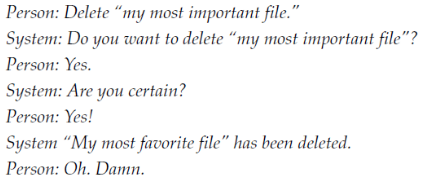
\includegraphics[scale=0.6]{immagini/Damn.png}
\end{figure}

Per prevenire errori è possibile quindi utilizzare:
\begin{itemize}
	\item \textbf{Constraints}: aggiungendo vincoli alle azioni. I sistemi elettronici hanno un'ampia selezione di metodi che possono essere usati per ridurre l'errore. Uno di questi può essere \textbf{segregare i controlli}, cosicché controlli confondibili tra loro vengano piazzati lontani l'uno dall'altro. Un altro è di \textbf{separare i moduli}, cosicché qualsiasi controllo non direttamente rilevante all'operazione corrente non sia visibile a schermo ma richieda uno sforzo extra per essere raggiunto.
	\item \textbf{Undo}: comando che annulla le operazioni effettuate dal precedente. I sistemi migliori hanno \textbf{più livelli di undoing} in modo tale da annullare intere sequenze di azioni.
	\item \textbf{Messaggi d'errore e di conferma}: molti sistemi cercano di prevenire l'errore chiedendo conferma prima di eseguire un comando, specialmente quando l'azione distruggerà qualcosa di importante. Tuttavia queste richieste sono spesso mal temporeggiate, perché \textbf{dopo aver richiesto un'operazione le persone sono solitamente certe di volerla compiere}. Un controllo migliore sarebbe visualizzare sia l'azione da compiere che l'oggetto interessato, con l'opzione annulla o prosegui.\textbf{ I messaggi di avviso sono sorprendentemente inefficaci contro gli errori}.

	\item  \textbf{Controlli di Sensibilità}: i sistemi elettronici presentano il vantaggio di poter controllare che l'operazione richiesta sia \textbf{sensibile} o \textbf{ragionevole}. Ad esempio verificare che l'importo indicato sia giusto, magari esponendo un avviso in caso di numeri eccessivamente grandi.
\end{itemize}

In estrema sintesi e ricollegandosi all'esempio della groviera, per ridurre gli errori si hanno le seguenti possibilità:

\begin{figure}[!h]
	\centering
	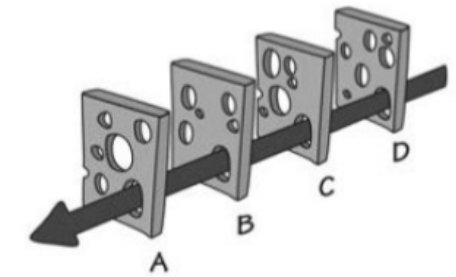
\includegraphics[scale=0.5]{immagini/Groviera.png}
\end{figure}

\begin{itemize}
	\item \textbf{Aumentare il numero di controlli} (le fette).
	\item \textbf{Migliorare il modello concettuale dell'utente}. (ridurre il numero di buchi, o rendere più piccoli i buchi esistenti, magari con un modello concettuale minimale e dei constraints)
	\item \textbf{Allertare l'operatore umano quando diversi buchi si allineano}.
\end{itemize}

\pagebreak



\pagebreak
